% bei Standalone in documentclass noch:
% \RequirePackage{luatex85}

\documentclass[captions=tableheading, titlepage= firstiscover, parskip = half , bibliography=totoc]{scrartcl}
%paper = a5 für andere optinen
% titlepage= firstiscover
% bibliography=totoc für bibdateien
% parskip=half  Veränderung um Absätze zu verbessern

\usepackage{scrhack} % nach \documentclass
\usepackage[aux]{rerunfilecheck}
\usepackage{polyglossia}
\usepackage[style=numeric, backend=biber]{biblatex} % mit [style = alphabetic oder numeric] nach polyglossia
\addbibresource{lit.bib}
\setmainlanguage{german}

\usepackage[autostyle]{csquotes}
\usepackage{amsmath} % unverzichtbare Mathe-Befehle
\usepackage{amssymb} % viele Mathe-Symbole
\usepackage{mathtools} % Erweiterungen für amsmath
\usepackage{fontspec} % nach amssymb
% muss ins document: \usefonttheme{professionalfonts} % für Beamer Präsentationen
\usepackage{longtable}

\usepackage[
math-style=ISO,    % \
bold-style=ISO,    % |
sans-style=italic, % | ISO-Standard folgen
nabla=upright,     % |
partial=upright,   % /
]{unicode-math} % "Does exactly what it says on the tin."
\setmathfont{Latin Modern Math}
% \setmathfont{Tex Gyre Pagella Math} % alternativ

\usepackage[
% die folgenden 3 nur einschalten bei documenten
locale=DE,
separate-uncertainty=true, % Immer Fehler mit ±
per-mode=symbol-or-fraction, % m/s im Text, sonst \frac
]{siunitx}

% alternativ:
% per-mode=reciprocal, % m s^{-1}
% output-decimal-marker=., % . statt , für Dezimalzahlen

\usepackage[
version=4,
math-greek=default,
text-greek=default,
]{mhchem}

\usepackage[section, below]{placeins}
\usepackage{caption} % Captions schöner machen
\usepackage{graphicx}
\usepackage{grffile}
\usepackage{subcaption}

% \usepackage{showframe} Wenn man die Ramen sehen will

\usepackage{float}
\floatplacement{figure}{htbp}
\floatplacement{table}{htbp}

\usepackage{mhchem} %chemische Symbole Beispiel: \ce{^{227}_{90}Th+}


\usepackage{booktabs}

 \usepackage{microtype}
 \usepackage{xfrac}

 \usepackage{expl3}
 \usepackage{xparse}

 % \ExplSyntaxOn
 % \NewDocumentComman \I {}  %Befehl\I definieren, keine Argumente
 % {
 %    \symup{i}              %Ergebnis von \I
 % }
 % \ExplSyntaxOff

 \usepackage{pdflscape}
 \usepackage{mleftright}

 % Mit dem mathtools-Befehl \DeclarePairedDelimiter können Befehle erzeugen werden,
 % die Symbole um Ausdrücke setzen.
 % \DeclarePairedDelimiter{\abs}{\lvert}{\rvert}
 % \DeclarePairedDelimiter{\norm}{\lVert}{\rVert}
 % in Mathe:
 %\abs{x} \abs*{\frac{1}{x}}
 %\norm{\symbf{y}}

 % Für Physik IV und Quantenmechanik
 \DeclarePairedDelimiter{\bra}{\langle}{\rvert}
 \DeclarePairedDelimiter{\ket}{\lvert}{\rangle}
 % <name> <#arguments> <left> <right> <body>
 \DeclarePairedDelimiterX{\braket}[2]{\langle}{\rangle}{
 #1 \delimsize| #2
 }

\setlength{\delimitershortfall}{-1sp}

 \usepackage{tikz}
 \usepackage{tikz-feynman}

 \usepackage{csvsimple}
 % Tabellen mit \csvautobooktabular{"file"}
 % muss in table umgebung gesetzt werden


% \multicolumn{#Spalten}{Ausrichtung}{Inhalt}

\usepackage{hyperref}
\usepackage{bookmark}
\usepackage[shortcuts]{extdash} %nach hyperref, bookmark

\newcommand{\ua}[1]{_\symup{#1}}
\newcommand{\su}[1]{\symup{#1}}

\title{Versuch 201}
\subtitle{Das Dulong-Petitsche Gesetz}
\author{Jonah Nitschke\\
        lejonah@web.de \and
        Sebastian Pape\\
        sepa@gmx.de}
\date{Durchführung: 29.11.2016\\
      Abgabe: 06.12.2016}

\begin{document}

\maketitle
\tableofcontents
\newpage

\section{Einführung}
Bei dem folgenden Versuch geht es darum, die Aussage des Dulong-Petitschen Gesetzes
über die Gleichmäßigkeit der Molwärme von verschiedenen Stoffen zu überprüfen und
darauf basierend zu Entscheiden, ob die klassische Mechanik zur Beschreibung
der oszillatorischen Bewegung von Atomen ausreicht oder ob dies nur auf der
Grundlage der Quantenmechanik geschehen kann.

\section{Theorie}

\subsection{\texorpdfstring{$\emph{spezifische Wärmekapazität}$}{z}}

Erhöht sich die Temperatur eines Körpers um $\increment T$ so ergibt sich
für aufgenommene Wärmeenergie und Temperaturdifferenz entsprechend
des 1. Thermodynamischen Hauptsatzes folgende Beziehung:

\begin{equation}
  \increment Q = m c \increment T
\end{equation}

Bei c handelt es sich dabei um die Wärmekapazität bzw. im Bezug auf den
vorliegenden Stoff um die \emph{spezifische Wärmekapazität}. Von
Bedeutung für das vorliegende Experiment ist zudem die \emph{Molwärme} C.
Sie beschreibt die benötigte Wärmemenge, um ein Mol eines Stoffes um dT zu
erwärmen. Dabei wird noch unter $C_V$ für konstante Volumen und $C_p$ für
konstanten Druck unterschieden.

\subsection{Dulong-Petit}

Das \emph{Dulong-Petitsche Gesetz} trifft die Aussage, dass die Atomwärme bei konstanten
Volumen $C_V$ im festen Aggregatzustand unabhängig von dem Charakter des Elements
ist, sondern konstant den Wert 3R annimmt (R = Allgemeine Gaskonstante). Die
Herleitung dieses Zusammenhanges basiert dabei auf der Annahme, dass Atome in
einem Festkörpergitter um feste Punkte schwingen, und ihre potentielle und
kinetische Energie dabei gleich sind. Gleichzeitig besagt das
\emph{Äquipartitionstheorem}, dass ein Atom dabei die kinetische Energie
$ \left< E_{kin} \right> = 1/2 k T$ besitzt. Aus beiden folgt dann für die mittlere Energie
des Festkörpers der Wert 3RT und aus diesem der oben geschriebene Wert für die
\emph{Molwärme} $C_V$.

Die Molwärme $C_V$ von allen festen chemischen Elementen nimmt bei hoher
Temperatur tatsächlich etwa den Wert 3R an, bei vielen Stoffen auch schon bei
Zimmertemperatur. Die kinetische Theorie kann allerdings nicht beschreiben, warum
die Molwärme aller chemischen Elementen bei hinreichend tiefen Temperaturen
beliebig klein wird.

Das liegt an der Annahme, dass die Energie der atomaren Oszillatoren sich
beliebig ändern kann. Dies steht im Widerspruch zu Quantentheorie, die
Energieänderungen nur in bestimmten Beträgen erlaubt. Die nun auf
komplizierte Weise von T abhängige mittlere Energie kann somit nur über
eine Aufsummierung der verschiedenen Energiezustände multipliziert mit der
jeweiligen Wahrscheinlichkeit ihres Auftretens geschehen. Mit der
Boltzmann-Verteilung ergibt sich für die innere Energie damit folgender Ausdruck:

\begin{equation}
  \left< U_{qu} \right> = \frac{ 3 N_l \hbar \omega}{\textbf{exp} (\hbar \omega / kT) - 1}
\end{equation}

Für den Grenzfall von $ T \to \infty$ ergibt sich jedoch auch hier wieder der
bekannte Zusammenhang von $\left< U_{qu} \right> = 3RT$.

\subsection{Messung der spez. Wärmekapazität fester Körper mit dem Mischungskalorimeter}

Da eine Messung mit konstantem Volumen schwer zu realisieren ist, wird bei dem
Experiment auf ein konstanten Druck zurückgegriffen. Dafür ist es notwendig, den
Zusammenhang zwischen $C_V$ und $C_p$ zu kennen:

\begin{equation}
  \label{eqn:Cp-CV}
  C_p - C_V = 9 \alpha^2 \kappa V_0 T
\end{equation}

Bei $\alpha$, $\kappa$ und $V_0$ handelt es sich um Konstanten. Für die abgegebene
Wärmeenergie des Körpers $(Q_1)$ und die aufgenommene Wärmemenge der Kalorimeterwände
ergeben sich folgende Formel:

\begin{align}
  Q_1 &= c_k m_k (T_k - T_m) \\
  Q_2 &= (c_W m_W + c_g m_g) (T_k - T_m)
\end{align}

Bei $T_m$ handelt es sich um die sich einstellende Mischtemperatur und alle Werte
mit Index k und W beziehen sich auf den Körper bzw. das Wasser.

Bei dem Experiment wird ein Wärmeverlust des Systems vernachlässigt, so dass
für die Bestimmung der spez. Wärmekapazität des Körpers die obigen Formeln
lediglich gleichgesetzt werden müssen $(Q_1=Q_2)$:

\begin{equation}
  \label{eqn:ck}
  c_k = \frac{(c_W m_W + c_g m_g) (T_k - T_m)}{m_k (T_k - T_m)}
\end{equation}

Die Wärmekapazität $c_g m_g$ des Kalorimeters muss am Anfang des Experiments
noch einmal extra bestimmt werden und kann mit folgender Formel errechnet werden:

\begin{equation}
  \label{eqn:cgmg}
  c_g m_g = \frac{c_W m_y \left(T_y - T_m' \right) - c_W m_x \left(T_x - T_m' \right)}{\left( T_m' - T_x \right)}
\end{equation}


\section{Messtechnische Hinweise}

Für die Messung der Temperaturen bei diesem Versuch wird ein Thermoelement benutzt.
Dies liegt vor allem and der sehr hohen Einstellgeschwindigkeit, die erzielt werden
kann. Das Thermoelement besteht aus zwei verschiedenen Metallen, die hinsichtlich
ihrer Elektronen-Austrittsarbeit unterschiedlich sind. Wie in Abbildung % Hier das Bild zum Thermoelement einfügen
zu erkennen, gibt es zwei Berührungstellen dieser Metalle. An diesen Berührungsstellen
wandern die Elektronen von dem Metall mit der niedrigeren in das Metall mit der
höheren Austrittsarbeit, bis das durch die Ladungsverschiebung entstehende Potential
diesen Elektronendrift unterbindet. Das enstehende Potenzial nennt man dann
\emph{Kontaktpotenzial}. Das Kontaktpotenzial hat an beiden Berührungstellen
allerdings ein anderes Vorzeichen, so dass an den Berührungsstellen der beiden
Metalle A keine Differenzspannung zu beobachten ist. Tritt nun an einer der beiden
Berührungsstelle eine Erwärmung auf, wird das Kontaktpotenzial beeinflusst und
die beiden Kontaktpotenziale heben sich nicht mehr auf. Daraus resultiert eine
messbare Spannung an den Enden der beiden A-Dräten, die spezifsch ist für jede
Temperaturdifferenz zwischen beiden Berührungsstellen.

\section{Durchführung}

Als erstes werden mithilfe der bereitstehenden Waage (Abbildung \ref{fig:Skizze}, 5)
die Massen der verschiedenen Körper bestimmt.

Bevor die Messungen für die \emph{spezifische Wärmekapazität} begonnen werden,
muss zuerst eine Referenzwert ermittelt werden, um hinterher mithilfe der gemessenen
Spannungen des Thermoelements (Abb. \ref{fig:Skizze}, 1) die vorliegenden Temperaturen zu bestimmen.
Dafür wird ein Dewar-Gefäß mit Eiswasser gefüllt (Abb. \ref{fig:Skizze}, 2) und in einem Becherglas
Wasser zum Kochen gebracht. Erst werden
beide Enden des Kabels in das Eiswasser gelegt, um die Spannungsdifferent bei
einem Temperaturunterschied von 0 K zu überprüfen. Anschließend wird ein Ende in
das kochende Wasser gelegt um die Spannungsdifferenz bei einem Unterschied von
100 K zu überprüfen. Mit beiden Spannungen kann ein lineare Regression ausgeführt
werden um die Paramter zur Bestimmmung der Temperatur in Abhängigkeit der
gemessenen Spannungen zu bestimmen.

Danach wird noch die die \emph{spezifische Wärmekapazität} des Kalorimeters bestimmt.
In das Dewar-Gefäß werden zwei Mengen an Wasser der Masse $m_x$ und $m_y$ und der
Temperaturen $T_x$ und $T_y$ gegeben. Anschließend wird die Mischtemperatur
$T_m$ gemessen und mit \eqref{eqn:cgmg} kann die \emph{spezifische Wärmekapazität}
bestimmt werden.

Nach den Vorbereitungen kann mit den eigentlichen Messungen gestartet werden.
Zuerst wird das Dewar-Gefäß mit der gleichen Flüssigkeitsmenge wie bei der
Bestimmung von $c_g m_g$ gefüllt (Abb. \ref{fig:Skizze}, 4). Dann wird das Blei in dem Becherglas mit kochendem
Wasser aufgeheizt (Abb. \ref{fig:Skizze}, 3). Dabei wird mit dem Thermoelement die Temperatur des Bleis
gemessen. Vor dem Eintauchen des Körpers in das Dewar-Gefäß wird die
Temperatur des Wassers noch einmal bestimmt. Nach einer kurzen Wartezeit wird
dann die Mischtemperatur gemessen.
Für die Metalle Blei 2 und Graphit wird die Messung drei mal durchgeführt.
Anschließend wird die Messung noch einmal für Kupfer durchgeführt.

\begin{figure}
  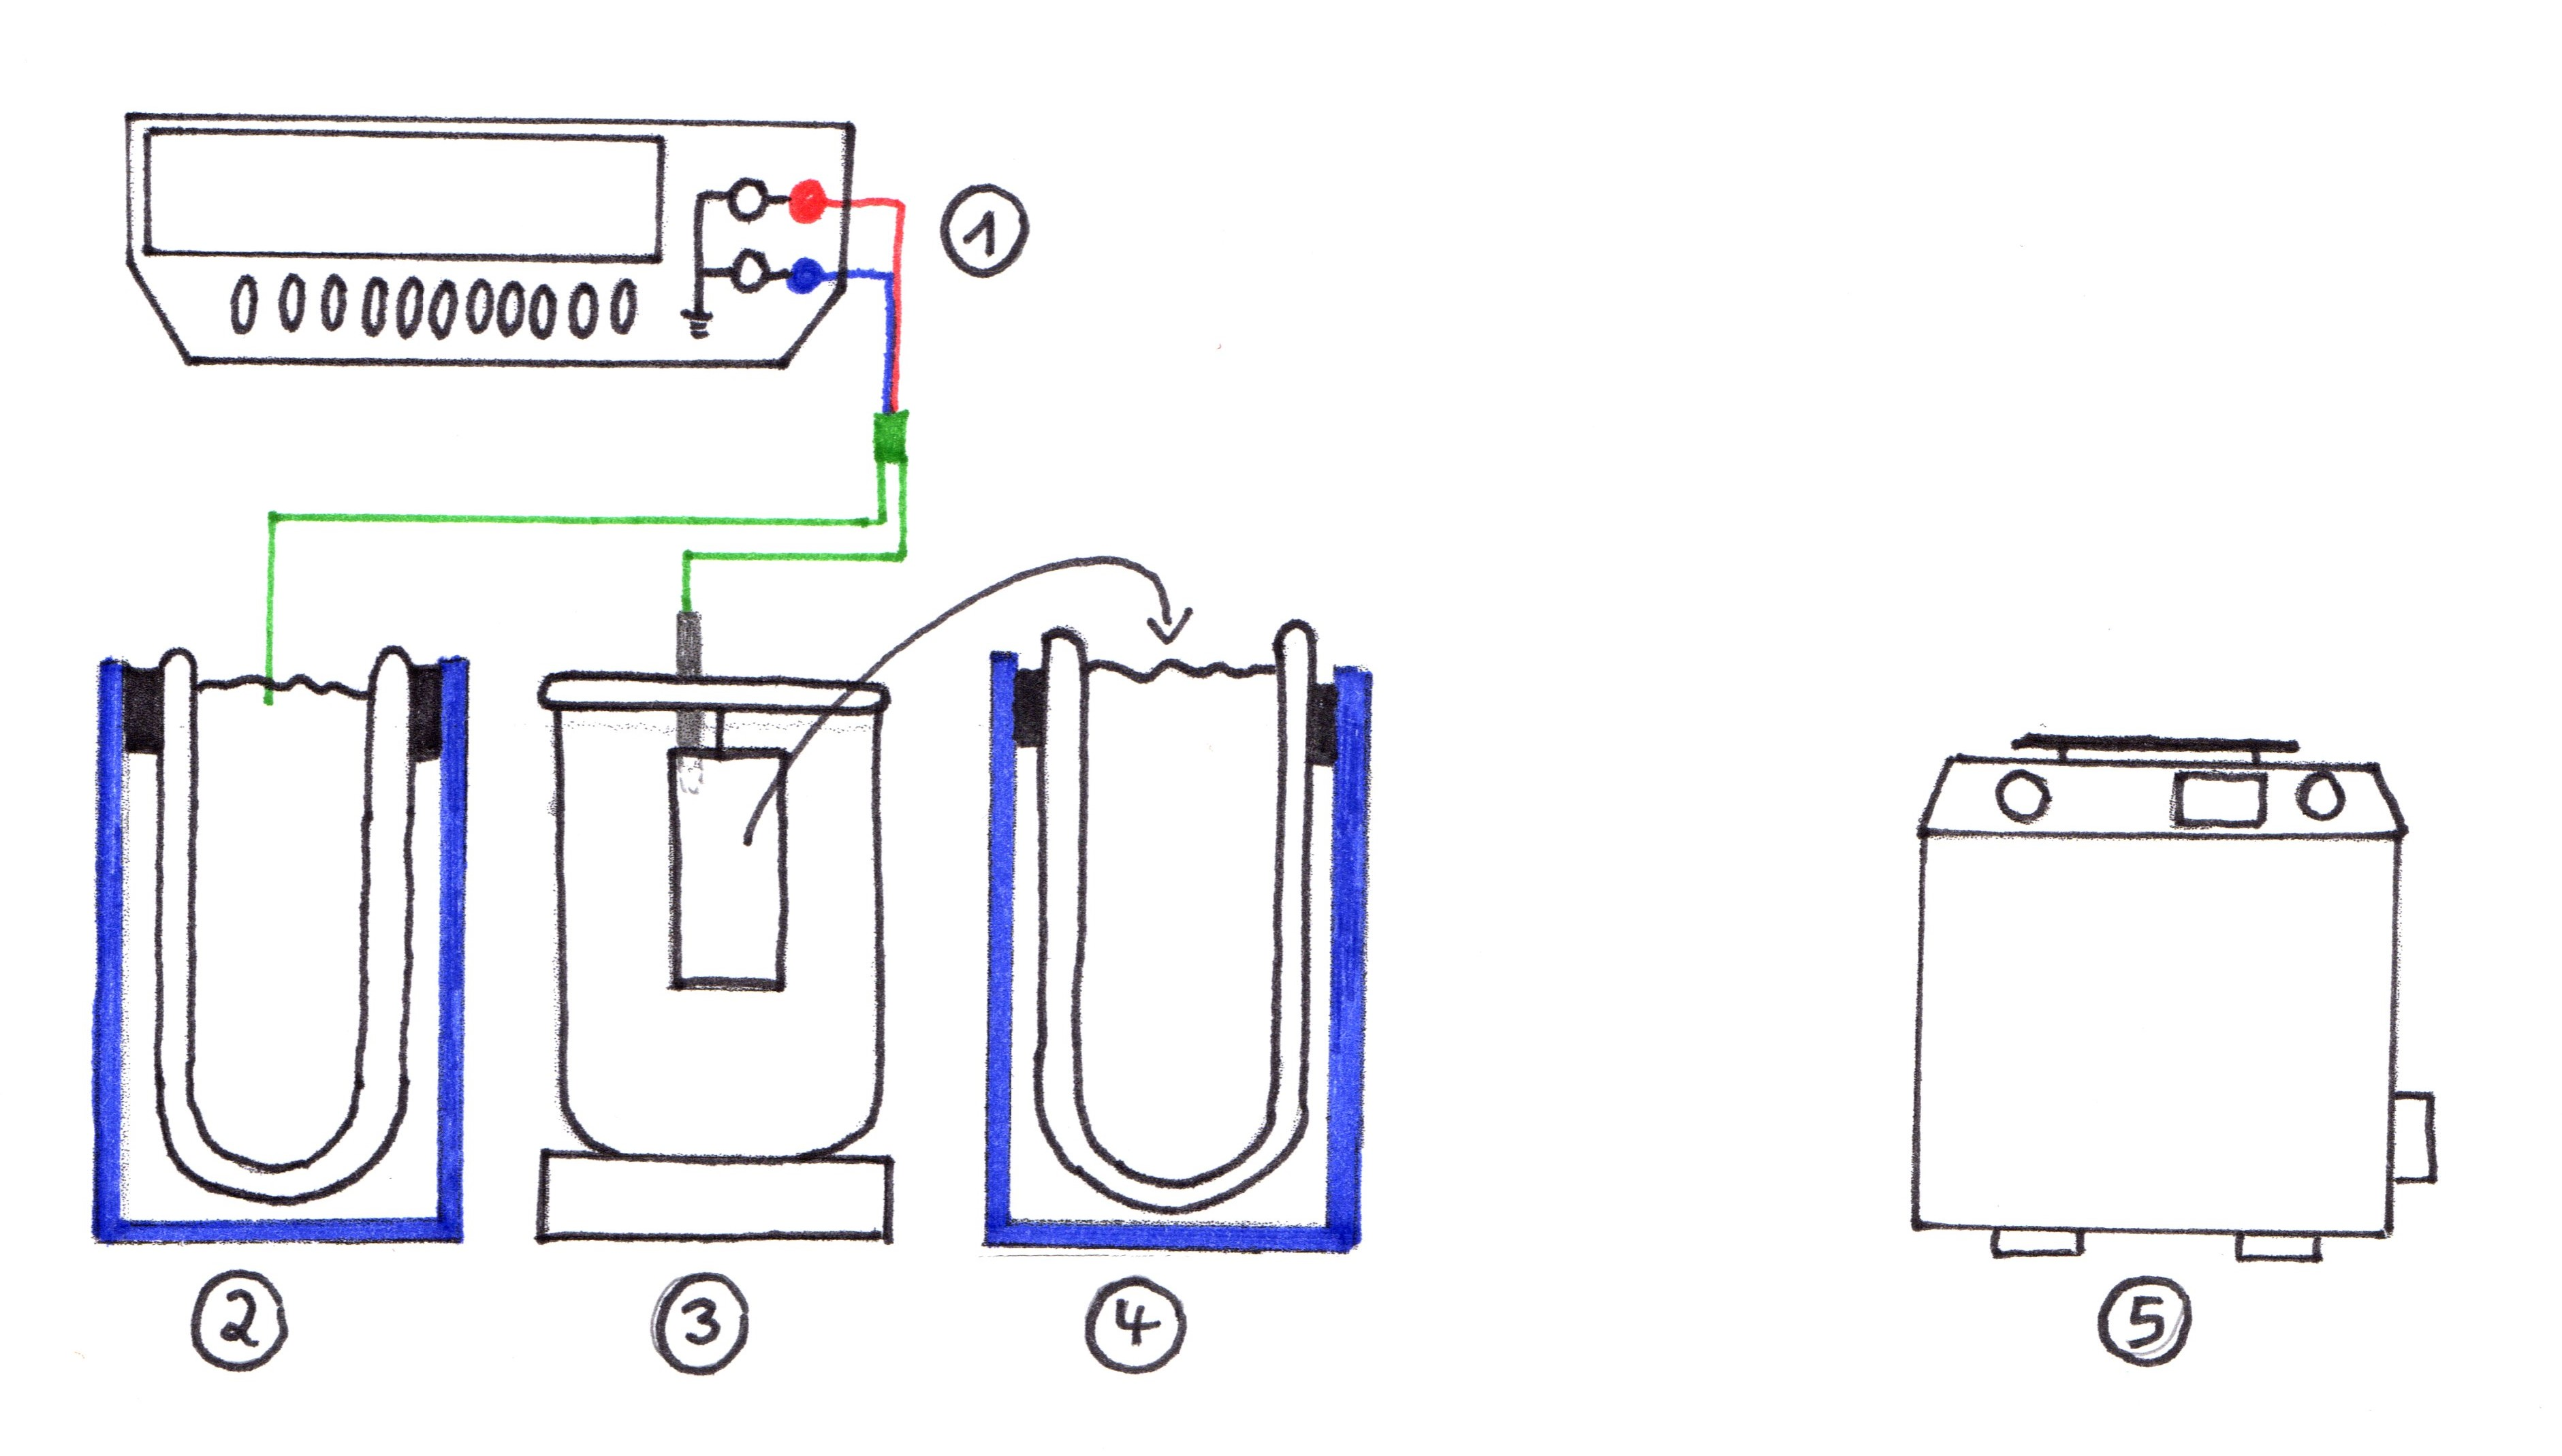
\includegraphics{VersuchsSkizze.jpg}
  \caption{Skizze des Versuchaufbaus}
  \label{fig:Skizze}
\end{figure}

\newpage

\section{Auswertung}

Alle Messergebnisse werden in zweistelliger Arithmetik angegeben. Zugehörige
Fehler sind auf sinnvoll erachtete Stellen gerundet.

\subsection{Justieren des Thermoelementes}
Zu Beginn des Veruches musste das Thermoelement justiert werden. Für die
Ausgleichgerade ergibt sich die folgende Funktion.

\begin{align*}
  T(U) &\approx 25.77 \cdot U + 273,15 & [T(U)] = \si{\kelvin}
\end{align*}

Die Funktion ist abhängig von den gemessenen Spannungen $U$ ($[U] = \si{\milli\volt}$).

\subsection{Bestimmen der spezifischen Wärmekapazität des Kalorimeters}

Zu Beginn des Versuches wurde die spezifische Wärmekapazität des Kalorimeters
$c_gm_g$ bestimmt, da diese Größe für die Berechnung der spezifischen
Wärmekapazität der Stoffe $c_k$ notwendig ist. Mittels Formel \eqref{eqn:cgmg} wurde
$c_gm_g$ ermittelt. Mit den folgenden Werten wurde $c_gm_g$ berechnet.

\begin{description}
  \item[$T_x$]$ = \SI{294,28}{\kelvin}$
  \item[$T_y$]$ = \SI{354,59}{\kelvin}$
  \item[$T_m$]$ = \SI{322,38}{\kelvin}$
  \item[$m_x$]$ = \SI{278,97}{\gram}$
  \item[$m_y$]$ = \SI{298,98}{\gram}$
\end{description}

Für die spezifische Wärmekapazität von Wasser wurde der Wert $c_w =
\SI{4,18}{\joule\per\gram\per\kelvin}$, wie in der Versuchsbeschreibung
\cite{anleitung} empfohlen verwendet.
Es ergibt sich ein Wert von $c_gm_g = \SI{267,09}{\joule\per\kelvin}$.

\subsection{Bestimmen der spezifischen Wärmekapazität von verschiedenen Stoffen}

Es wurden in dem Versuch die spezifische Wärmekapazität der Stoffe Graphit,
Blei und Kupfer bestimmt, wobei für Blei die Probe Blei 2 verwendet wurde.
Für Graphit und Blei wurden jeweils drei Messungen und für Kupfer lediglich eine
Messung durchgeführt. Die spezifische Wärmekapazität $c_k$ eines Körpers
wird über Formel \eqref{eqn:ck} ermittelt. In der beiliegenden Tabelle sind die gemessenen
Größen des jeweiligen Stoffes eingetragen.

\floatplacement{table}{htpb}
\begin{table}
 \centering
 \label{tab:Messdaten1}
 \begin{tabular}[width=0.4\textwidth]{S S[table-format=3.2] S[table-format=3.2]
   S[table-format=3.2] S[table-format=3.2]}
     \toprule
     {}  & {$T_w$ in $\si{\kelvin}$} & {$T_k$ in $\si{\kelvin}$} &
     {$T_m$ in $\si{\kelvin}$} & {$m_w$ in $\si{\gram}$} \\
     \midrule
     \text{Graphit} & & & & \\
     \text{Messung 1} & 293,77 & 377,27 & 296,09 & 772,50 \\
     \text{Messung 2} & 297,38 & 374,44 & 299,70 & 772,50 \\
     \text{Messung 3} & 299,95 & 375,45 & 302,53 & 772,50 \\
     & & & & \\
     \text{Blei} & & & & \\
     \text{Messung 1} & 295,31 & 371,60 & 296,86 & 765,89 \\
     \text{Messung 2} & 296,86 & 369,28 & 298,41 & 765,89 \\
     \text{Messung 3} & 298,41 & 370,57 & 299,95 & 765,89 \\
     & & & & \\
     \text{Kupfer} & & & & \\
     \text{Messung 1} & 293,77 & 377,79 & 294,80 & 769,56 \\
     \bottomrule
\end{tabular}
  \caption{Messdaten der verwendeten Stoffe}
\end{table}
\FloatBarrier

Für die untersuchten Proben ergibt sich somit:

\begin{align*}
  c_{Graphit} &= (\num{1,02 +- 0,064})\si{\joule\per\gram\per\kelvin} \\
  c_{Blei} &= (\num{0,19 +- 0,004})\si{\joule\per\gram\per\kelvin} \\
  c_{Kupfer} &= \num{0,18}\si{\joule\per\gram\per\kelvin} \\
\end{align*}

Die Fehler für Graphit und Blei wurden über die folgende Formel bestimmt.

\begin{equation}
  \label{eqn:Fehler}
  \increment\bar{x} = \sqrt{\frac{1}{N(N - 1)}
  \cdot\sum_{i = 1}^N(x_i-\bar{x})^2}
\end{equation}

Dabei ist $\bar{x}$ der Mittelwert der gemessenen Größe.

\subsection{Bestimmen der Atomwärme}

Damit die Atomwärme $C_p$ eines Stoffes bestimmt werden kann, muss die
spezifische Wärmekapazität dieses mit seiner Molarenmasse multipliziert werden.

\begin{equation}
  C_p = c_k\cdot M
\end{equation}

Für den jewiligen Stoff ergibt sich somit:

\begin{align*}
  C_{pG} &= (\num{12,29 +- 0,768})\si{\joule\per\mol\per\kelvin} \\
  C_{pB} &= (\num{39,99 +- 0,727})\si{\joule\per\mol\per\kelvin} \\
  C_{pK} &= \num{11,50}\si{\joule\per\mol\per\kelvin}
\end{align*}

\subsection{Vergleich mit Dulong-Petit}

Aus den Überlegungen der klassischen Mechanik, die bereits in der Theorie
erwähnt wurden ergibt sich, dass die Atomwärme $C_V$ materialunabhängig
und konstant den Wert $3\cdot R \approx \SI{24,94}{\joule\per\mol\per\kelvin}$
beträgt. Nun gilt es diese Aussage zu überprüfen.
Der Zusammenhang zwischen $C_p$ und $C_V$ ist nach Formel \eqref{eqn:Cp-CV} bekannt.
In der folgenden Tabelle sind die berechneten Werte von $C_V$, sowie ihre
prozentuale Abweichung von dem Theoriewert aus dem \emph{Dulong-Petitschen
Gesetz}. Die Werte wurden anhand der Daten aus der Versuchbeschreibung
\cite{anleitung} berechnet.

\floatplacement{table}{htpb}
\begin{table}
 \centering
 \label{tab:Vergleich}
 \begin{tabular}[width=0.4\textwidth]{S S[table-format=2.2] S[table-format=1.4]
 S[table-format=2.2]}
     \toprule
     {} & {$C_V$ in \si{\joule\per\mol\kelvin}}  & {$\increment C_V$ in
     $\si{\joule\per\mol\kelvin}$} & {\small{Prozentuale Abweichung}} \\
     \midrule
     \text{Graphit} & 12,26 & 0,0002 & \text{--}49,15 \\
     \text{Blei} & 38,26 & 0,0052 & \text{+}53,39 \\
     \text{Kupfer} & 10,78 & \text{\,\,\,\,\,\,\,\,\,\,\,\textbf{---}} & \text{--}43,22 \\
     \bottomrule
   \end{tabular}
  \caption{Vergleich zwischen dem \emph{Dulong-Petitschen Gesetz}
  und den gemessenen Werten}
\end{table}

\section{Diskussion}

In dem Versuch wurde überprüft, ob eine klassische Betrachtung der Ozillation
von Atomen in einem Festkörper möglich ist, oder ob dies bereits mit Hilfe
der Quantenmechanik angegangen werden muss. Die Aussage kann anhand der
Vergleichswerte von $C_V$ mit $3R$ getroffen werden. Aus diesen folgt, dass
die Oszillation der Atome in Festkörpern quantenmechanisch betrachtet werden
muss, da die Messergebnisse deutlich von den Theoriewert verschieden sind.
Dabei ist jedoch zu sagen, dass die Messungenauigkeiten in dem Versuch nicht
zu vernachlässigen sind. Die Sicherheit der Ergebnisse  wurde deutlich von der
Qualität des Thermoelements beschnitten. Zum einen wurde die hundert Grad Marke,
die bei der Justierung bestimmt wurde teilweise von den erhitzten Proben
überschritten. Solch eine Überschreitung zeigt, dass die zuvor bestimmte
Eichmarke fehlerhaft war. Dies bedeutet, dass jede Temperaturmessung mit einem
systematischen Fehler behaftet ist. Zum anderen hatte das Thermoelement
unberechenbare Fehlfunktionen, weshalb die Genauigkeit und Zuverlässigkeit des
Thermoelementes in Frage zustellen ist. Die Restlichen Messgrößen, wie das
Gewicht der Proben konnte porblemlos bestimmt werden. Es ist anzunehmen, dass
abgesehen von der Temperaturmessung die restlichen Größen keinen systematischen
Fehler unterliegen. Anhand der aufgeführten Argumente kann die Aussage
weder wiederlegt, noch bestätigt werden.

\printbibliography

\end{document}
